\documentclass[11pt,aspectratio=169]{beamer}

\usepackage{amsmath,amssymb,bm}
\usepackage{graphicx}
\usepackage{booktabs}
\usepackage{listings}

\usetheme{default}
\setbeamertemplate{navigation symbols}{}
\setbeamertemplate{headline}{}
\setbeamertemplate{footline}{}
\setbeamertemplate{frametitle}{%
  \vspace{0.25cm}%
  \insertframetitle\par
  \vspace{0.08cm}%
  \hrule
}
\setbeamercolor{normal text}{fg=black,bg=white}
\setbeamercolor{frametitle}{fg=black,bg=white}
\setbeamercolor{structure}{fg=black}
\setbeamersize{text margin left=0.7cm,text margin right=0.7cm}

\newcommand{\dd}{\,\mathrm{d}}
\newcommand{\Ke}{\mathcal K_e}
\newcommand{\Ee}{\mathcal E}
\newcommand{\bK}{\bm K}
\newcommand{\bF}{\bm F}
\newcommand{\bU}{\bm U}
\newcommand{\bR}{\bm R}

\lstset{
  language=Python,
  basicstyle=\ttfamily\scriptsize,
  keywordstyle=\bfseries,
  commentstyle=\itshape,
  showstringspaces=false,
  columns=fullflexible,
  keepspaces=true,
  frame=single,
  framerule=0.3pt,
  xleftmargin=0.2em,
  xrightmargin=0.2em,
  aboveskip=0.4em,
  belowskip=0.2em
}

\graphicspath{{figures/}}

\begin{document}

\begin{frame}[plain]
  \centering
  \vfill
  {\LARGE\bfseries Finite Element Assembly\par}
  \vspace{0.45cm}
  {\large One-dimensional linear elements\par}
  \vfill
\end{frame}

\section{Local and global finite element quantities}

\begin{frame}{What assembly must accomplish}
For the axial bar,
\[
  \int_0^L AE\,u_h'v_h'\dd x
  =
  \int_0^L f v_h\dd x+\overline P\,v_h(L).
\]

Each element supplies a small matrix and vector,
\[
  \bK^e
  =\int_{\mathcal K_e}(\bm B^e)^T AE\,\bm B^e\dd x,
  \qquad
  \bF^e
  =\int_{\mathcal K_e}(\bm N^e)^T f\dd x.
\]

Assembly must place these local entries into the correct rows and columns of
\[
  \bK\bU=\bF.
\]
\end{frame}

\begin{frame}{Local and global node numbers}
  \centering
  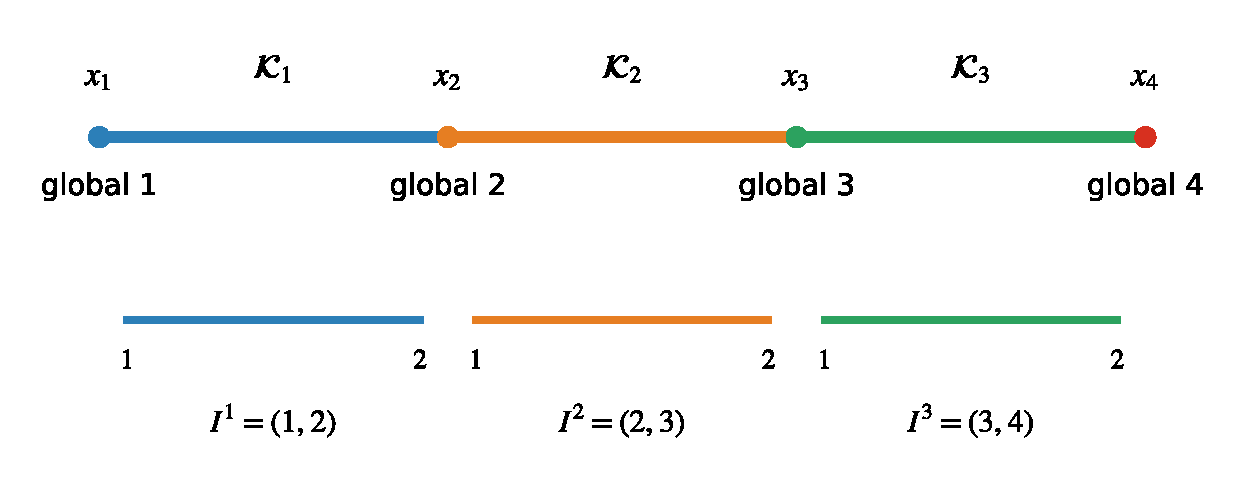
\includegraphics[width=0.94\textwidth]{local_global_numbering.pdf}

  \vspace{0.2cm}
  Local node numbers restart on each element. Global node numbers identify
  shared nodes of the complete mesh.
\end{frame}

\begin{frame}{The three maps used in assembly}
For a two-node element,
\[
  I^e:\{1,2\}\longrightarrow\{1,\ldots,N+1\},
  \qquad
  I^e(1)=e,\quad I^e(2)=e+1.
\]

For a global node that belongs to element $e$,
\[
  J^e:\{I^e(1),I^e(2)\}\longrightarrow\{1,2\},
  \qquad
  J^e(I^e(a))=a.
\]

The elements incident on global node $i$ are
\[
  \mathcal E(i)=
  \{e:x_i\in\overline{\mathcal K}_e\}.
\]

For the shared node $2$,
\[
  J^1(2)=2,
  \qquad
  J^2(2)=1,
  \qquad
  \mathcal E(2)=\{1,2\}.
\]
\end{frame}

\begin{frame}{Local support determines the interacting basis functions}
  \centering
  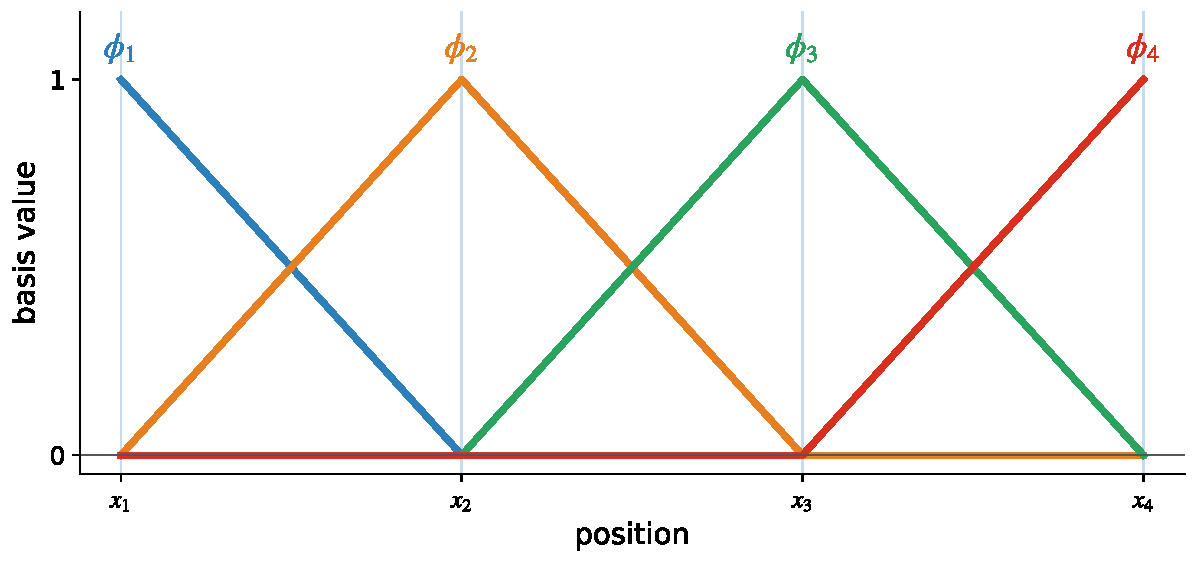
\includegraphics[width=0.72\textwidth]{global_linear_basis.pdf}

  \vspace{0.15cm}
  \[
    \operatorname{supp}\phi_i
    =\bigcup_{e\in\mathcal E(i)}\overline{\mathcal K}_e.
  \]

  On element $e$, only the basis functions associated with its two nodes are
  nonzero.
\end{frame}

\begin{frame}{A global function restricted to one element}
The global finite element function is
\[
  u_h(x)=\sum_{i=1}^{N+1}U_i\phi_i(x).
\]

On $\mathcal K_e$, all terms except those associated with its two nodes vanish:
\[
  u_h|_{\mathcal K_e}
  =U_{I^e(1)}\phi_1^e+U_{I^e(2)}\phi_2^e
  =\bm N^e\bU^e,
\]
where
\[
  \bU^e=
  \begin{bmatrix}
    U_{I^e(1)}\\[2pt]U_{I^e(2)}
  \end{bmatrix}.
\]

Connectivity extracts the local coefficient vector from the global vector.
\end{frame}

\section{Assembly of the global system}

\begin{frame}{Load-vector assembly by global entry}
The distributed part of global entry $i$ is
\[
  F_i^{\mathrm{dist}}
  =\sum_{e=1}^{N}\int_{\mathcal K_e}f\phi_i\dd x.
\]

Only elements in $\mathcal E(i)$ contribute. Define
\[
  F_a^e=\int_{\mathcal K_e}f\phi_a^e\dd x.
\]
Since $\phi_i|_{\mathcal K_e}=\phi_{J^e(i)}^e$,
\[
  \boxed{
  F_i^{\mathrm{dist}}
  =\sum_{e\in\mathcal E(i)}F_{J^e(i)}^e.}
\]

This formula fixes a global node $i$ and gathers all incident-element
contributions.
\end{frame}

\begin{frame}{Three-element load vector}
For
\[
  I^1=(1,2),\qquad I^2=(2,3),\qquad I^3=(3,4),
\]
the distributed-load vector is
\[
  \bF^{\mathrm{dist}}
  =
  \begin{bmatrix}F_1^1\\F_2^1\\0\\0\end{bmatrix}
  +
  \begin{bmatrix}0\\F_1^2\\F_2^2\\0\end{bmatrix}
  +
  \begin{bmatrix}0\\0\\F_1^3\\F_2^3\end{bmatrix}
  =
  \begin{bmatrix}
    F_1^1\\
    F_2^1+F_1^2\\
    F_2^2+F_1^3\\
    F_2^3
  \end{bmatrix}.
\]

At a shared node, the neighboring element contributions add.
\end{frame}

\begin{frame}{Stiffness-matrix assembly by global entry}
The global entry is
\[
  K_{ij}
  =\sum_{e=1}^{N}
  \int_{\mathcal K_e}AE\,\phi_j'\phi_i'\dd x.
\]

An element contributes only if it contains both nodes $i$ and $j$. With
\[
  K_{ab}^e
  =\int_{\mathcal K_e}AE\,(\phi_b^e)'(\phi_a^e)'\dd x,
\]
we obtain
\[
  \boxed{
  K_{ij}
  =\sum_{e\in\mathcal E(i)\cap\mathcal E(j)}
  K_{J^e(i),J^e(j)}^e.}
\]

For example,
\[
  K_{22}=K_{22}^1+K_{11}^2,
  \qquad K_{23}=K_{12}^2,
  \qquad K_{14}=0.
\]
\end{frame}

\begin{frame}{Three-element stiffness matrix}
  \centering
  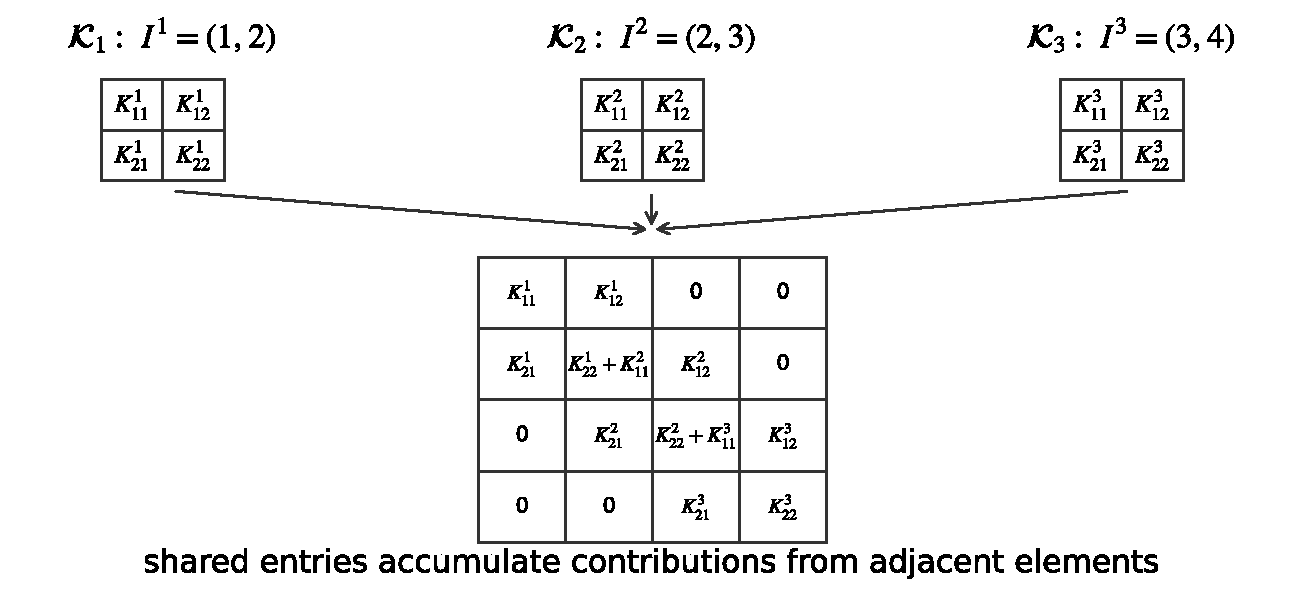
\includegraphics[width=0.95\textwidth]{assembly_scatter_add.pdf}
\end{frame}

\begin{frame}[fragile]{The assembly operation used in code}
The entry formulas gather contributions for a fixed global index. A program
usually loops over elements and scatters local entries:
\[
  \boxed{
  F_{I^e(a)}\mathrel{+}=F_a^e,
  \qquad
  K_{I^e(a),I^e(b)}\mathrel{+}=K_{ab}^e.}
\]

\begin{lstlisting}
for e in range(num_elements):
    dofs = connectivity[e]
    K_e, F_e = element_arrays(e)

    for a in range(2):
        F[dofs[a]] += F_e[a]
        for b in range(2):
            K[dofs[a], dofs[b]] += K_e[a, b]
\end{lstlisting}

The arrays use zero-based Python indices. The mathematical map $I^e$ uses
one-based indices.
\end{frame}

\section{Boundary conditions and reactions}

\begin{frame}{Essential boundary conditions}
  \centering
  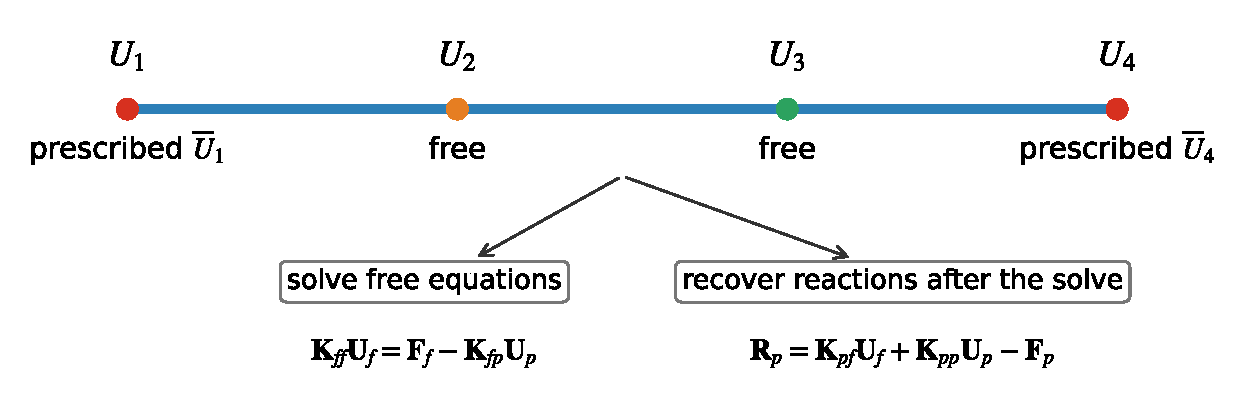
\includegraphics[width=0.88\textwidth]{essential_bc_partition.pdf}

  \vspace{0.1cm}
  With free indices $f$ and prescribed indices $p$,
  \[
    \bK_{ff}\bU_f
    =\bF_f-\bK_{fp}\bU_p.
  \]

  Solve only for the free coefficients, then insert the prescribed values into
  the complete vector $\bU$.
\end{frame}

\begin{frame}{Reactions and final checks}
After constructing the complete coefficient vector,
\[
  \bR=\bK\bU-\bF.
\]

The entries associated with prescribed degrees of freedom are the reactions:
\[
  \bR_p
  =\bK_{pf}\bU_f+\bK_{pp}\bU_p-\bF_p.
\]

Before accepting the solution, check:
\begin{itemize}
  \item the connectivity and element lengths;
  \item the free and prescribed degree-of-freedom sets;
  \item global equilibrium using applied loads and reactions;
  \item displacement and axial-force trends against the loading.
\end{itemize}
\end{frame}

\begin{frame}{Complete finite element procedure}
\begin{enumerate}
  \item Create node coordinates and element connectivity.
  \item Initialize the global matrix $\bK$ and vector $\bF$.
  \item For each element, compute $\bK^e$ and $\bF^e$.
  \item Scatter-add the element entries using $I^e$.
  \item Separate free and prescribed degrees of freedom.
  \item Solve the reduced system for $\bU_f$.
  \item Insert prescribed values and compute reactions.
  \item Evaluate displacement, strain, stress, and axial force elementwise.
\end{enumerate}
\end{frame}

\section{Numerical demonstration and error measures}

\begin{frame}{Notebook demonstration problem}
Set $L=AE=f_0=1$ and solve
\[
  -u''=1\quad\text{in }(0,1),
  \qquad
  u(0)=0,
  \qquad
  u'(1)=0.
\]

The exact solution is
\[
  u(x)=x-\frac{x^2}{2}.
\]

During the demonstration:
\begin{itemize}
  \item assemble and inspect $\bK$ and $\bF$ for one mesh;
  \item impose the essential boundary condition and solve;
  \item examine the displacement error; and
  \item then introduce derivative-based errors and mesh refinement.
\end{itemize}
\end{frame}

\begin{frame}[fragile]{Element loop in the demonstration}
For uniform linear elements with $h=x_{e+1}-x_e$,
\[
  \bK^e=\frac{1}{h}
  \begin{bmatrix}1&-1\\-1&1\end{bmatrix},
  \qquad
  \bF^e=\frac{h}{2}
  \begin{bmatrix}1\\1\end{bmatrix}.
\]

\begin{lstlisting}
for e in range(num_elements):
    dofs = np.array([e, e + 1])
    h_e = nodes[e + 1] - nodes[e]

    K_e = np.array([[1.0, -1.0],
                    [-1.0, 1.0]]) / h_e
    F_e = 0.5 * h_e * np.ones(2)

    for a in range(2):
        F[dofs[a]] += F_e[a]
        for b in range(2):
            K[dofs[a], dofs[b]] += K_e[a, b]
\end{lstlisting}
\end{frame}

\begin{frame}[fragile]{Solve, recover the reaction, and compare}
\begin{lstlisting}
num_nodes = len(F)
U = np.zeros(num_nodes)
K_ff = K[1:, 1:]
F_f = F[1:]
U[1:] = np.linalg.solve(K_ff, F_f)

reaction = (K @ U - F)[0]
\end{lstlisting}

For this problem, the computed nodal values agree with the exact quadratic
solution at the nodes. Between nodes, $u_h$ is piecewise linear. Mesh
refinement reduces the interpolation error.
\end{frame}

\begin{frame}{Begin with the displacement error}
Let $e=u-u_h$. We first examine errors in the solution values:
\[
  \lVert e\rVert_{L^2}
  =\left(\int_0^1e^2\dd x\right)^{1/2},
  \qquad
  \lVert e\rVert_{\infty}
  =\max_{x\in[0,1]}|e(x)|.
\]

For this problem, $u_h$ agrees with $u$ at the nodes. The exact solution is
quadratic, while $u_h$ is linear on each element. The error therefore vanishes
at the nodes but is nonzero inside each element.

For linear elements in this particular problem,
\[
  \lVert e\rVert_{L^2}=O(h^2),
  \qquad
  \lVert e\rVert_{\infty}=O(h^2).
\]
\end{frame}

\begin{frame}{Energy and $H^1$ errors}
The preceding norms do not measure the derivative error. For the bar problem,
\[
  \lVert e\rVert_E
  =\left(\int_0^1AE(e')^2\dd x\right)^{1/2},
\]
while
\[
  \lVert e\rVert_{H^1}
  =\left(\lVert e\rVert_{L^2}^2
  +\lVert e'\rVert_{L^2}^2\right)^{1/2}.
\]

Here $AE=1$, so the energy norm is the $H^1$ seminorm. Since $e(0)=0$,
the energy and $H^1$ norms are equivalent by the Poincar\'e inequality.

For linear elements and this smooth solution,
\[
  \lVert e\rVert_E=O(h),
  \qquad
  \lVert e\rVert_{H^1}=O(h).
\]
\end{frame}

\begin{frame}{Analysis in the notebook}
For one mesh, the notebook displays:
\begin{itemize}
  \item the finite element and exact solutions in the left panel;
  \item the pointwise absolute error in the right panel; and
  \item the $L^2$ and supremum errors in the error-plot title.
\end{itemize}

Only after interpreting these errors do we compute the energy and $H^1$
errors. The mesh-refinement loop then displays:
\begin{itemize}
  \item all finite element solutions with the exact solution; and
  \item all four error norms against $h$ on log--log axes.
\end{itemize}

For this problem, the fitted slopes should be approximately $2$ for the
$L^2$ and supremum errors and approximately $1$ for the energy and $H^1$
errors.
\end{frame}

\end{document}
